\documentclass[12pt]{article}
\usepackage[english]{babel}
\usepackage[english]{isodate}
\usepackage[table,svgnames]{xcolor}
\usepackage{url}
\usepackage[utf8x]{inputenc}
\usepackage[T1]{fontenc}
\usepackage{longtable}
\usepackage{amsmath}
\usepackage{graphicx}
\usepackage{parskip}
\usepackage{fancyhdr}
\usepackage{vmargin}
\usepackage{hyperref}
\usepackage{pgfgantt}
\usepackage{pgf-umlcd}
\usepackage{xparse}
\usepackage{float}
\usepackage{tabularx}
\usepackage{titling}
\usepackage{fancyhdr}
\usepackage{listings}
\usepackage{pdflscape}
\bibliographystyle{fontysIEEtranN}

% Global graphiscspath
\graphicspath{{../../../img/}}

% Styling changes

%% Better margins
\setmarginsrb{3 cm}{2.5 cm}{3 cm}{2.5 cm}{1 cm}{1.5 cm}{1 cm}{1.5 cm}


\begin{document}
	\begin{titlingpage}
		\begin{center}
			\begin{minipage}{\linewidth}
				\centering
				%University logo
				
\includegraphics[width=0.3\linewidth]{FontysLogo.pdf}
				\par
				\vspace{3cm}
				%Thesis title
				{\uppercase
					{\Large Quality Management Plan \\ 2015 Sofa GTL \\ TreeWatch Project
						\par
						\vspace{3cm}}}
				
\includegraphics[width=0.5\linewidth]{TreewatchLogo.pdf}
				\par
				\vspace{2cm}
				%Author's name
				{Jan Kerkenhoff\\
					Martijn Bonajo\\
					Max van der Linden\\
					René Karoff\\
					Ron Gebauer
					\par}
				\vspace{2cm}
				
				%Date
				\today
			\end{minipage}
		\end{center}
	\end{titlingpage}
	\clearpage
\section*{Document information}
\begin{tabular}{ll}
	\textbf{Document name:} & Quality Management Plan\\
	\textbf{Document owner:} & TreeWatch \\
	\textbf{Company/Organisation:} & Fleuren Baarlo \\
	\textbf{Contact person:} & Max van der Linden, Group leader \\
	\textbf{Date:} & \today \\
	\textbf{Place:} & Fontys University of Applied Science Venlo \\
	\textbf{Authors:} & \parbox[t]{5cm}{
		Jan Kerkenhoff\\ j.kerkenhoff@student.fontys.nl\\ 2197164 \\ \\
		Martijn Bonajo\\ m.bonajo@student.fontys.nl\\ 2213297 \\ \\
		Max van der Linden\\ max.vanderlinden@student.fontys.nl\\ 2209349 \\ \\
		René Karoff\\ r.karoff@student.fontys.nl\\ 2198664 \\ \\
		Ron Gebauer\\ r.gebauer@student.fontys.nl\\ 2153294 \\ }
\end{tabular}
\clearpage
\listoffigures
\addcontentsline{toc}{section}{\listfigurename}
\listoftables
\addcontentsline{toc}{section}{\listtablename}
\pagebreak

\tableofcontents
\clearpage

\section{Introduction}
This quality management plan describes the necessary information needed to manage the project quality from the project planning to the delivery to the customer. Within this document the quality policies, procedures, roles, responsibilities and authorities are defined.
\clearpage
\section{Organization and Responsibilities}
The SoFa Group consists of five people. Since the SoFa Group should act as a company roles and responsibilities have to be defined.\\
The following table shows every group member with his role and the responsibilities.
\begin{table}[htbp]
	\begin{tabularx}{\textwidth}{ X X X }
		\textbf{Name} & \textbf{Role} & \textbf{Quality Responsibility} \\ \hline
		Max van der Linden & Project Manager & Project Planning, External communication, Auditing \\ 
		Martijn Bonajo & Configuration Manager & Configuration Plan, Infrastructure, Approve Packages and Pushes to Master, Auditing \\ 
		Ron Gebauer & Scrum Master & Scrum planning, Auditing \\ 
		Rene Karoff & Quality Manager & Quality Management Plan, Ensure use of quality guidelines, Auditing \\ 
		Jan Kerkenhoff & Main Engineer & Main Code-Master, Auditing \\
	\end{tabularx}
	\caption{Group roles\label{tab:GroupRoles}}
\end{table}
Besides his role, the group will work together on several tasks (e.g. User Stories, Design or Implementation).
\clearpage
\section{Quality Planning}
This chapter is about the defined project quality standards and how the project standards are measured. The defined standards include coding style guides as well as documentation style guides.

\subsection{Define Project Quality}
Since this project is about programming a mobile business application, it is highly important that the system has a minimum of bugs/errors. A good documentation is necessary too, not only because this application will be developed by VAA ICT Consultancy after the SoFa is finished, but the customer should understand the system which is developed.
To ensure that the quality of the written code it matches the expectation of our customer it is mandatory to develop every module test-driven, therefore unit-testing is introduced. The written documents will be checked for its grammar, writing style and content.\\
Furthermore there are several design constraints which every member of the group has to follow when creating a document, these constraints are defined in the chapter Quality assurance.

\subsection{Measure Project Quality}
During the implementation every implemented feature needs to be reviewed by another group member, the written code is reviewed and if there is any effect on the GUI, it is also to be reviewed. 

In the Appendix is a table which contains the description which document was reviewed by whom and what grade (from \textcolor{red}{- -} to \textcolor{green}{++}) it got when it was approved.

The code of the application will be tested. Therefore it is a goal to get at least 90\% code coverage, better 100\%. 
\clearpage
\section{Quality Assurance}
Since the code is tested, this will show the group if the quality goal is achieved. Furthermore the written documents will be audited by at least one group member and the project quality manager. This chapter also contains the Writing guidelines as well as the used coding convention.
\subsection{Writing Guidelines}
\begin{description}
	\item[General] Each document which will be created shall be created using LaTeX
	\item[Template] Every document which will be created shall use a Template containing:
	\subitem Titlepage
	\subitem Document information
	\item[Fontsize] The Font size for default text is 12pt, LaTeX scales the headings according to the default text size.
	\item[Date format] The Date in every documents to be written in according to ISO 8601
	\subitem use \verb|\today| or \verb|\printdate{dd.mm.yyyy}|
	\item[Tables \& Figures] Tables and Figures shall be marked as what they are
	\subitem use \verb|\caption{Guidelines \label{tab:Guidelines}}|
	\item[Images] Images inside a document shall be readable when printed, if images are to big, the have to be in the appendix
	\item[Documents to be delivered] Every document which is sent to anyone, will be exported as a .PDF-File
	\item[Citations] Citations are to be done with the IEEE standard which is also used within the Fontys Internship reports and the Graduation reports
	
\end{description}

		\subsection{Coding convention}
		To keep the code readable and understandable it is important that every programmer uses the same coding convention which is hereby defined as the official Microsoft C\# Coding Conventions. \cite{Microsoft}
		
		\section{Analyze Project Quality}
		Since this project is this application is implemented with Xamarin, the group wasn't able to find a suitable possibility to measure the code coverage, however within Xamarin it should be possible somehow to introduce code coverage measurements since it uses the Mono-framework but due to several forums (e.g. \cite{CodeCoverage}) It would take a lot of effort and consume a lot of time which the group prefers to spend on the solution. Furthermore the writer of a document will receive feedback of the auditing persons, so he can improve on his writing too.
		\clearpage
		\section{Improve Project Quality}
		To improve the quality of code the following tools were used:
		\begin{description}
			\item[Pair programming] Writing code with the 4-eyes-principle helps preventing errors especially with complicated algorithms.
			\item[Feature-driven development] Every developer o devloper pair implements one feature and only if this feature works correctly the next feature will be implemented.
			\item[Test-driven devlopment] In order to have the code working properly, the code was tested using unit-testing
		\end{description}
		\clearpage
		\section{Quality Control}
		To verify that the quality of every document and every feature matches the introduced standard they were reviewed by at least one group member, therefore the review process shown in Figure~\ref{reviewProcess} was introduced. In the review process the term 'document' is defined as either a .PDF-document or a feature.
		\begin{figure}[htpb]
			\minipage{\textwidth}
			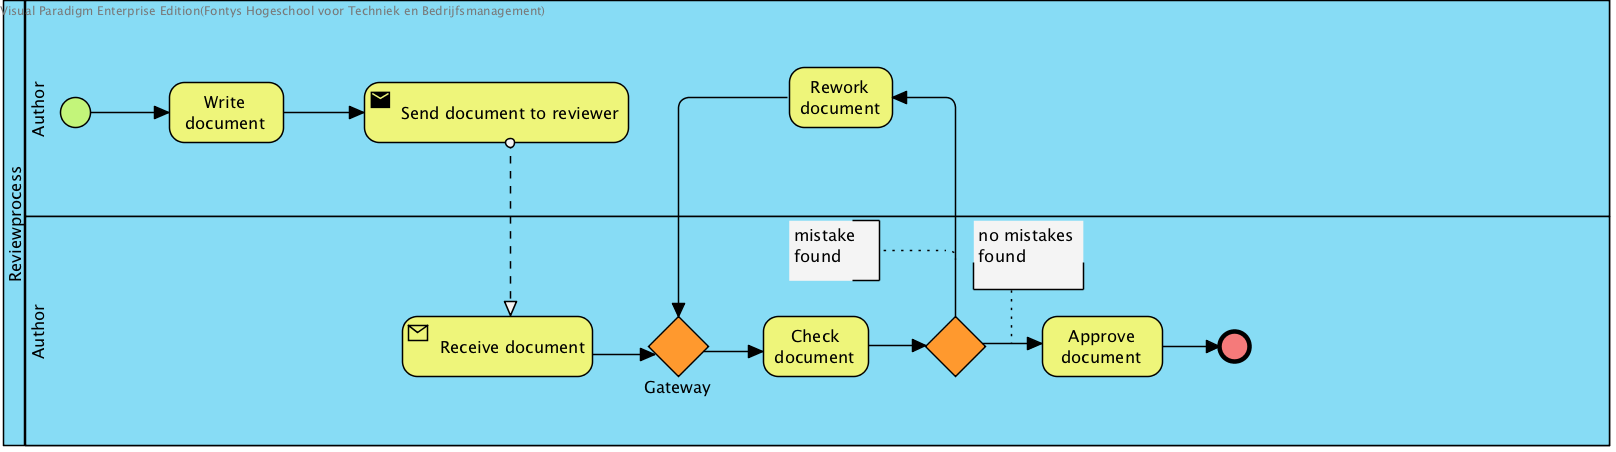
\includegraphics[width=\linewidth, keepaspectratio=true]{./img/CheckQuality.png}
			\caption{Review Process}\label{reviewProcess}
			\endminipage\hfill
		\end{figure}
		\clearpage
\bibliography{biblist}
\clearpage
\section{Appendix}
\begin{sidewaystable}
	\section*{Appendix}
	\subsection*{Reviewed Documents}
		\begin{longtable}[htbp]{ l p{3.7cm} *{2}{l} p{3.7cm} l}
			\textbf{Document} & \textbf{Author} & \textbf{Reviewer} & \textbf{Grade} & \textbf{Remark} & \textbf{Approval}\\ \hline
			Native vs Hybrid & Rene Karoff \& Martijn Bonajo & Jan Kerkenhoff &+& & yes\\
			SCRUM Planning & Ron Gebauer & & & & \\
			Quality Management Plan & Rene Karoff & Max van der Linden &-&  Add reviewed documents& no \\
			Quality Management Plan & Rene Karoff & Max van der Linden &+& & yes \\
			Configuration Plan & Martijn Bonajo & Jan Kerkenhoff &-& Add Git-Structure & no\\
			Configuration Plan & Martijn Bonajo & Jan Kerkenhoff &+&  & yes\\
			ER Diagram & Rene Karoff & Martijn Bonajo & - & Spelling Error& No\\
			ER Diagram & Rene Karoff & Martijn Bonajo &++&& Yes\\
			User Stories & Max van der Linden & Group \& Customer & ++ & & yes \\
			Mockups & Groupwork & Customer & 0 & No grade given &  yes\\
		\end{longtable}
		\captionof{table}{All Reviewed Documents\label{tab:ReviewedDocuments}}
\end{sidewaystable}
\end{document}
